LIGO interferometers use several high finesse optical cavities for gravitational wave 
detection. The lengths of these cavities are controlled using radio frequency 
(RF) modulation-demodulation techniques in a Pound-Drever-Hall (PDH) locking scheme 
\cite{Black01}.  
This scheme provides an error signal that is linear to cavity length over a 
specific range. This study examines the specific case of the triangular ring cavity 
uses in LIGO interferometers for input mode cleaning. When the length of the cavity 
approaches the boundaries of the PDH error signal linear range, our model of the 
input mode cleaner PDH response shows that the resulting error signal contains 
non-linear spectral artifacts. This model and understanding of the non-linear 
cavity responses will be useful in the commissioning phase of the Advanced LIGO 
project for more precisely locating and eliminating systematic noise sources in 
the interfereometers

\section{PDH locking}

Resonance in an optical cavity is achieved when the round-trip length of the 
cavity is equal to an integer number of wavelengths of the input beam,
\begin{equation}
L = N\lambda = \frac{Nc}{\nu}
\end{equation}
where L is the round-trip length of the optical cavity, $\lambda$ is the 
wavelength of the light, $\nu$ is the frequency of the light, and c is the 
speed of light. 
Under these conditions, the light circulating in the cavity
will be in phase and add constructively, resulting in an optical gain that
increases the intracavity power. This is the state in which the LIGO 
optical cavities are intended to operate.
If we invert this equation, the allowed 
frequencies of light for which resonance will occur is then 
\begin{equation}
\nu = N\frac{c}{L}.
\end{equation}
The spacing between these allowed frequencies is called the free spectral 
range, 
\begin{equation}
\nu_\mathrm{FSR} = \frac{c}{L}.
\end{equation}
When the frequency of the light is equal to an integer multiple of 
the free spectral range, the system will be on resonance. This is, 
however, a delicate condition to maintain. If the frequency of the light 
changes while the cavity length is stable, the optical field will no longer 
overlap perfectly within the cavity 
and the incident light will be reflected. If the length of the optical cavity 
changes but the frequency is stable, the geometry of the cavity and the optical 
field will once again be mismatched and resonance will be lost. 
This can be thought of as the free spectral range of the cavity varying with L 
while the carrier beam frequency is constant. 
To solve this problem, LIGO 
employs feedback loops that use a PDH error signal to maintain the resonance 
condition. We will use the LIGO input mode cleaner as an example of PDH locking.

The Advanced LIGO input mode cleaner is a resonant triangular ring cavity used to isolate 
the TEM00 mode of the input beam. The geometry of the cavity is designed such that 
higher order modes of the optical field will be reflected and not transmitted to 
the rest of the interferometer. The carrier beam, however, will be resonant in 
the input mode cleaner and will be transmitted. To control the input mode cleaner, 
the reflected 
light incident on the input mode cleaner is read out on a photodiode. The reflected 
part of the carrier beam, which on resonance should be highly transmitted, 
is compared to the reflected part of an RF sideband which should be highly 
reflected.

The first necessary piece of information to generate the PDH error signal is 
the reflectivity of the optical cavity as a function of frequency. This function 
will have minima at integer multiples of the free spectral range, where the 
cavity is on resonance and light is circulating in the cavity. As the frequency 
of the light drifts, the reflectivity of the cavity will increase, rejecting more 
of the incident light. For the IMC, 
the reflection function is 
\begin{equation}
F(\omega) = \frac{r(1 + e^{-i\phi})}{1+r^2e^{-i\phi}} = \frac{r(1 + e^{-i(\frac{\omega}{\nu_{fsr}})})}{1+r^2e^{-i(\frac{\omega}{\nu_{fsr}})}}
\end{equation}
where $\omega$ is the frequency of the light, $r$ is the reflection coefficient 
of the input mirror, $\phi$ is the round-trip phase 
accumulated as the light propagates through the cavity, 
and $\nu_{\mathrm{FSR}}$ is the free spectral range of the cavity \cite{Mueller}.
This function returns a complex value, the amplitude and phase represent the 
amplitude and phase of the reflected field relative to the field incident to 
the cavity.

Figure \ref{fig:imc-reflection} shows the reflected amplitude and phase of 
the carrier beam and the 24 MHz RF sideband relative to the incident optical 
fields. For this demonstration, 
we will assume that the frequency of the light is stabilized and the 
x-axis represents a change in free spectral range due to a change in 
cavity length. That is, the x-axis is linearly related to the length of the 
optical cavity. 
When the cavity length matches the input beam, the reflectivity is minimized and the 
carrier is transmitted through the IMC. The sideband, which is at a higher frequency, 
is by design not resonant in the cavity and is fully reflected.
As the cavity length deviates from the resonance length, the reflected amplitude and 
phase of the carrier 
beam will change along with it. However, the reflected amplitude and phase of the 
RF sideband, which is not resonant in the IMC, are not sensitive to changes in 
cavity length around the resonance point.

\begin{figure}[h!]
\centering
  \subfloat{
  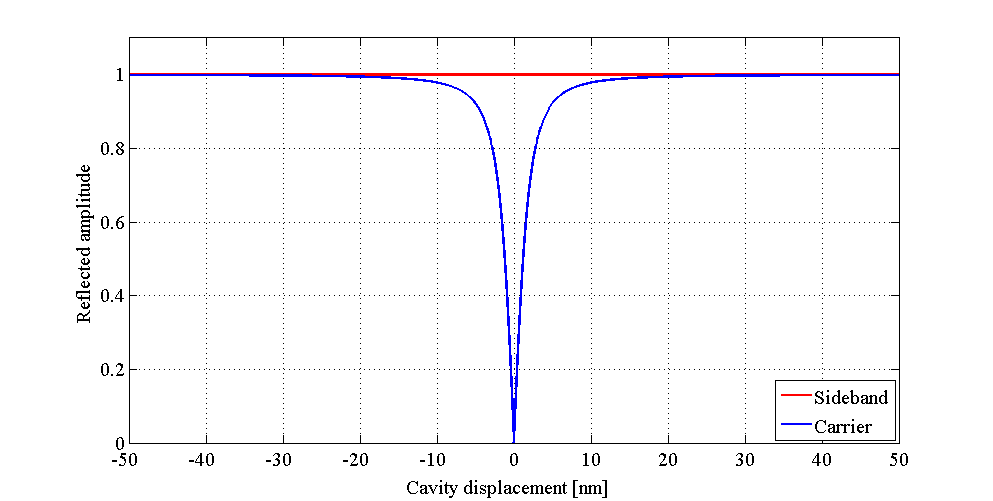
\includegraphics[width=\textwidth]{figures/IMCUpconversion/reflectivity}
  \label{fig:reflectivity}
  }

  \subfloat{
  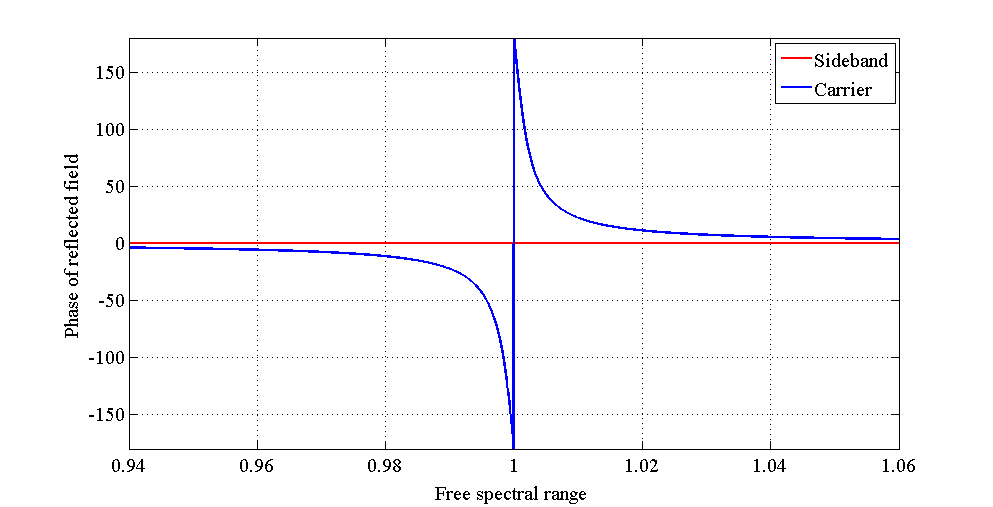
\includegraphics[width=\textwidth]{figures/IMCUpconversion/reflected-phase}
  \label{fig:reflected-phase}
  }
\caption[Reflection at the IMC]{Amplitude and phase of light reflected from %
         the IMC relative to the incident optical field. The amplitude reflectivity %
         is at a minimum when the cavity is on resonance, allowing the carrier beam %
         to be transmitted into the interferometer. The amplitude and phase of the %
         carrier beam will change as the cavity length changes. The amplitude %
         and phase of the RF sideband are not sensitive to changes in the cavity %
         length. This information can be used to generate an error signal that %
         represents the length of the input mode cleaner.}
\label{fig:imc-reflection}
\end{figure}

Using the function for the complex reflection coefficient, the reflected light 
can be read out on a photodiode and used to generate an 
error signal that is linear to the length of the cavity within a certain range. 
In a situation where the carrier beam is resonant in the cavity and the RF 
sidebands are high enough in frequency that they are not resonant, the PDH error 
signal is
\begin{equation}
\epsilon(\omega) = -2\sqrt{P_{c}P_{s}}\operatorname{Im}\{F(\omega)F^*(\omega + \Omega) - F^*(\omega)F(\omega - \Omega)\},
\end{equation}
where $P_{c}$ is the the carrier beam power and $P_{s}$ is the sideband power 
\cite{Black01}.
Figure \ref{fig:pdh} shows the resulting PDH error signal as a function of 
the free spectral range with an overlaid straight line as a reference for 
linearity. Looking at a zoomed in view of the error signal around the the linear 
part, we can see that the PDH signal matches the linear reference very well 
up to $\pm0.0005$ of a free spectral range.

\begin{figure}[h!]
\centering
  \subfloat{
  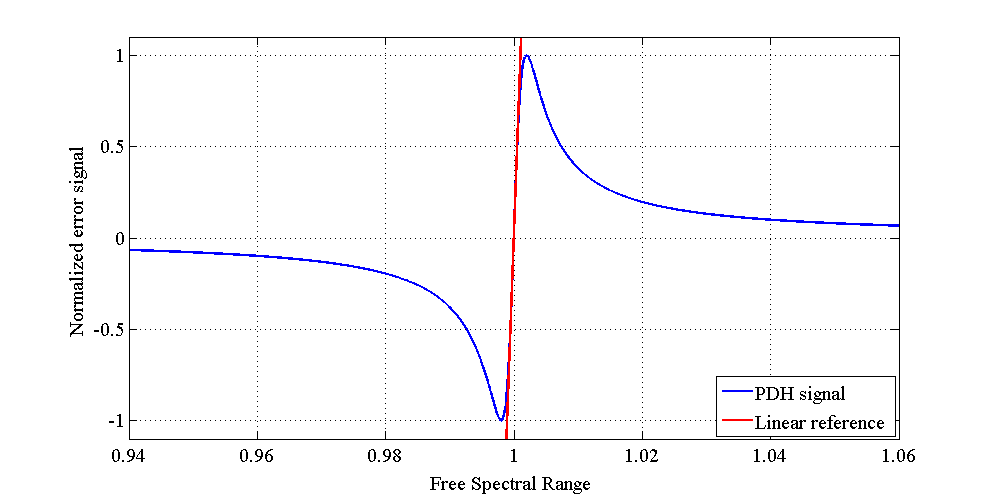
\includegraphics[width=\textwidth]{figures/IMCUpconversion/linear-pdh}
  \label{fig:regular-pdh}
  }

  \subfloat{
  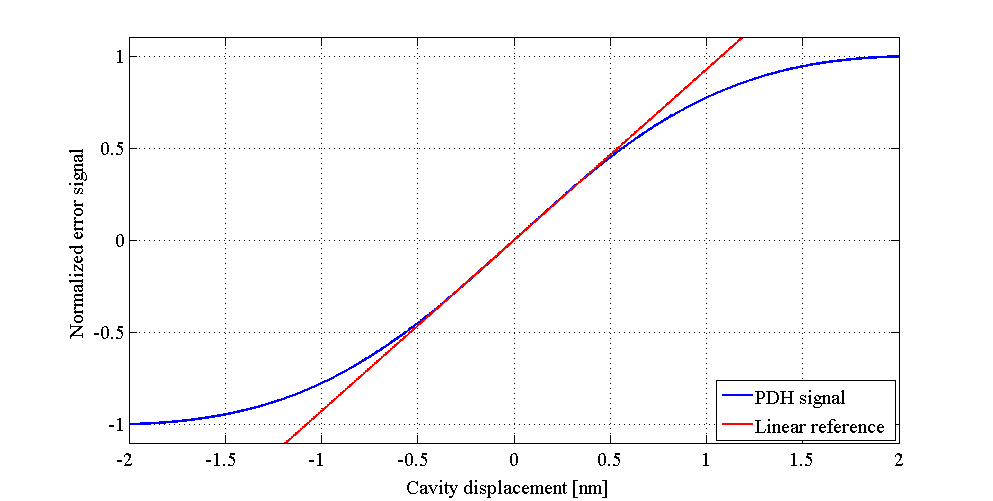
\includegraphics[width=\textwidth]{figures/IMCUpconversion/zoomed-pdh}
  \label{fig:zoom-pdh}
  }
\caption[Example of a PDH error signal]{Example of a PDH error signal. %
         The x-axis in this plot is linearly related to the length of the %
         input mode cleaner. 
         The red line is a straight line reference to estimate the linearity %
         of the error signal. %
         The error signal is linear to the length of the %
         input mode cleaner up to $\pm0.0005$ of a free spectral range. Motion %
         beyond this point will begin to contain non-linear artifacts and %
         eventually reach a turning point where control of the optics is lost.}
\label{fig:pdh}
\end{figure}

If the cavity motion exceeds this linear range, the error signal will 
contain non-linear artifacts which will bleed into the control signal 
used to actuate on the cavity optics.
To explore this non-linearity, we injected a sinusoidal cavity motion into our 
model and observed the resulting error signal.
The frequency of the sine wave was selected in an attempt to model 
noise seen in the output of the interferometers.  
The PDH response of the cavity was modeled using measured values of optical 
reflectivity and free spectral range of the Livingston input mode cleaner. 
The input beam was the nominal LIGO carrier beam with a frequency of 
$\omega = 281.8$ THz ($\lambda = 1064$ nm) and modulation sidebands of 
$\Omega = \pm24$ MHz.

We explored two specific cases. Figure \ref{fig:asymmetric-pdh} shows the 
power spectral density of the injected sinusoidal 
cavity motion (green) and the resulting non-linear error signal (blue). 
This motion was injected asymetrically about the nominal cavity locking point 
($\epsilon = 0$). The effect of this non-linearity is to take the injected 
sine wave and produce an error signal that looks like a sine wave with a 
flattened top, resembling a mixture of a pure sine wave with a square wave. 
Thus, we see both even and odd harmonics of the injection frequency when the 
signal is observed in the frequency domain.

Figure \ref{fig:symmetric-pdh} shows the power spectral density of the injected 
sinusoidal cavity motion (green) and the 
resulting non-linear error signal (blue). However, this time the motion was 
injected symetrically about the nominal cavity locking point. The resulting 
error signal was similar to a square wave and as a result 
we only see odd harmonics of the fundamental frequency.

\begin{figure}[h!]
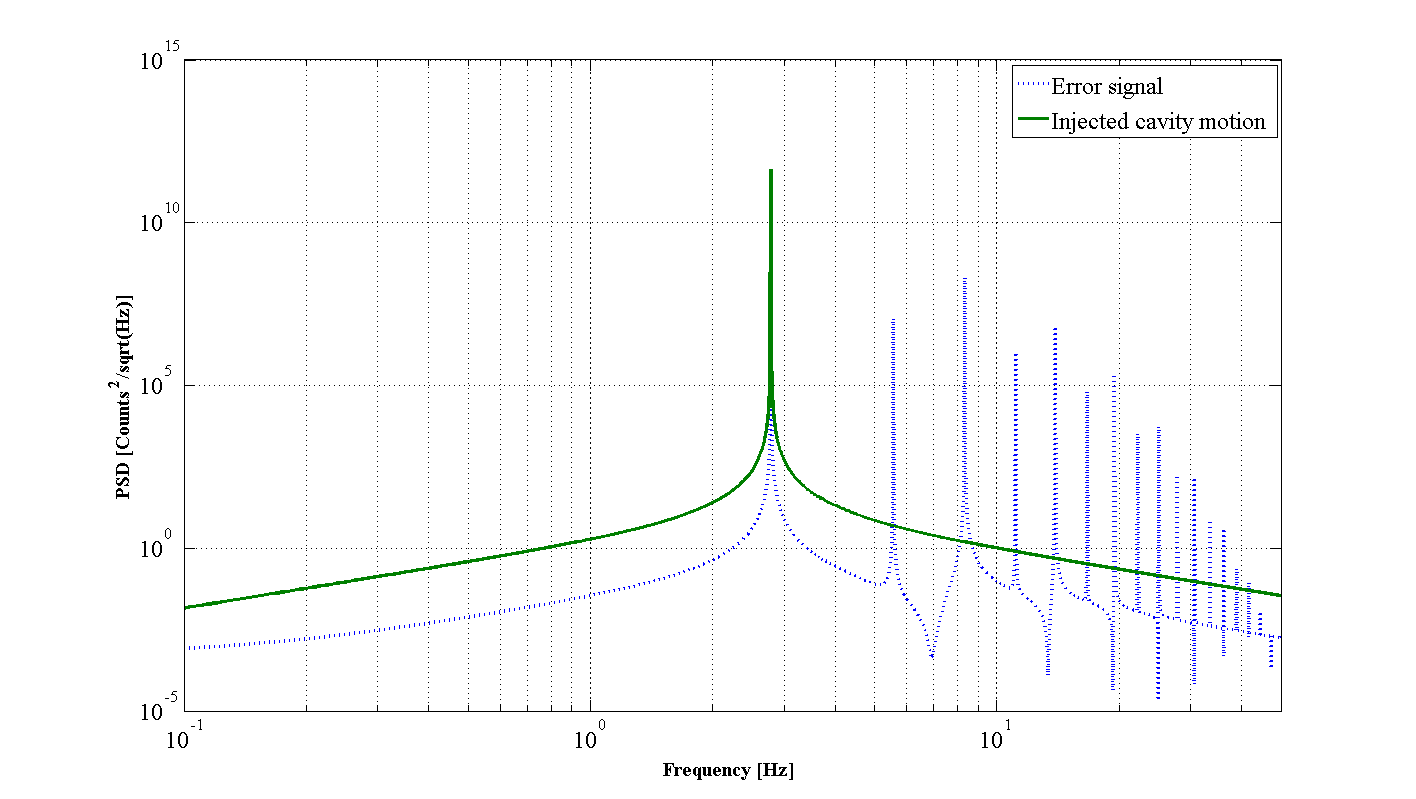
\includegraphics[height=0.6\textwidth]{figures/IMCUpconversion/PDH_error_signal_harmonics.png}
\caption[PDH response to asymmetric cavity motion]{Sinusoidal cavity motion with frequency 2.78 Hz injected asymmetrically about the locking point of the cavity results in a PDH error signal containing non-linear spectral artifacts at harmonics of the injected cavity motion.}
\label{fig:asymmetric-pdh}
\end{figure}

\begin{figure}[h!]
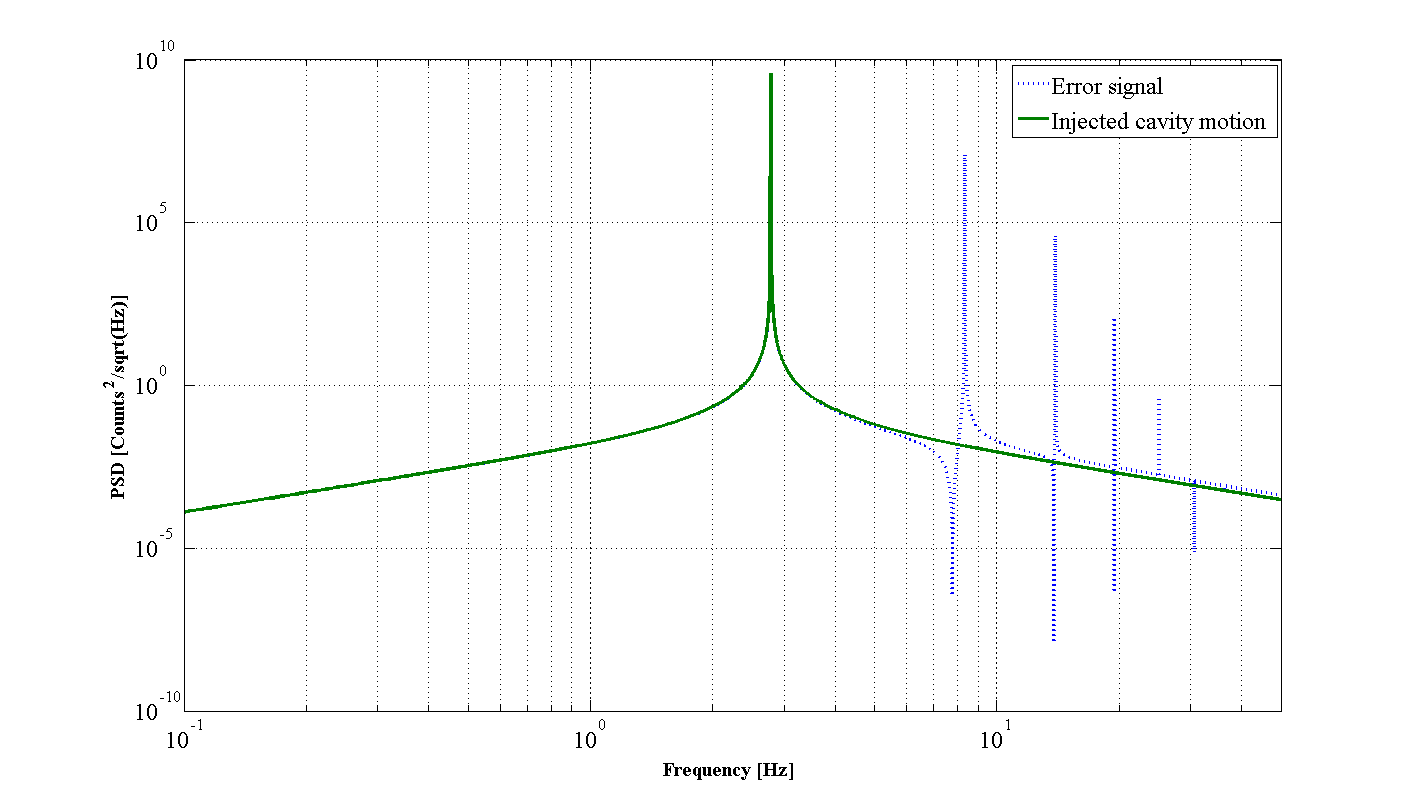
\includegraphics[height=0.6\textwidth]{figures/IMCUpconversion/symmetric_PDH.png}
\caption[PDH response to symmetric cavity motion]{If the motion is symmetric about the cavity locking point, we see only odd harmonics of the injection frequency.}
\label{fig:symmetric-pdh}
\end{figure}

\section{Upconversion noise in aLIGO}
Each of the three mirrors in the input mode cleaner cavity is staged as the bottom 
mass of a triple suspension in order to passively isolate the mirrors from noise. 
In addition, the chambers holding the IMC mirrors are isolated from ground motion by 
two stages of active seismic isolation. This isolation, however, is not completely 
impervious to external excitations. During periods of time with excess ground motion 
we can see seismic noise coupling into the cavity length and its control signal.

Specifically, when we see excess seismic noise in the 1-5 Hz anthropogenic band, 
believed to be caused by a commercial railroad a few kilometers from the LIGO 
Livingston, we see highly structured noise in the IMC control signal in the 10-100 Hz 
band. This physical mechanism is consistent with the model of a non-linear PDH error 
signal. If excess seismic motion reaches the suspension and the optics begin swinging 
around, it's feasible that they could start to saturate the linear range of the PDH loop.

The noise takes a form very similar in structure to the non-linear PDH signal, displaying 
strong odd harmonics and weaker even harmonics. The IMC control signal has an associated 
noise floor that obscures parts of these peaks. The theoretical model uses sinusoids with 
a highly specified frequency and thus displays very sharp peaks in its spectrum. 
It should be noted that the peaks in the IMC control signal are the manifestation of 
a physical process, not digitally generated, and have some natural width to them.

\begin{figure}[h!]
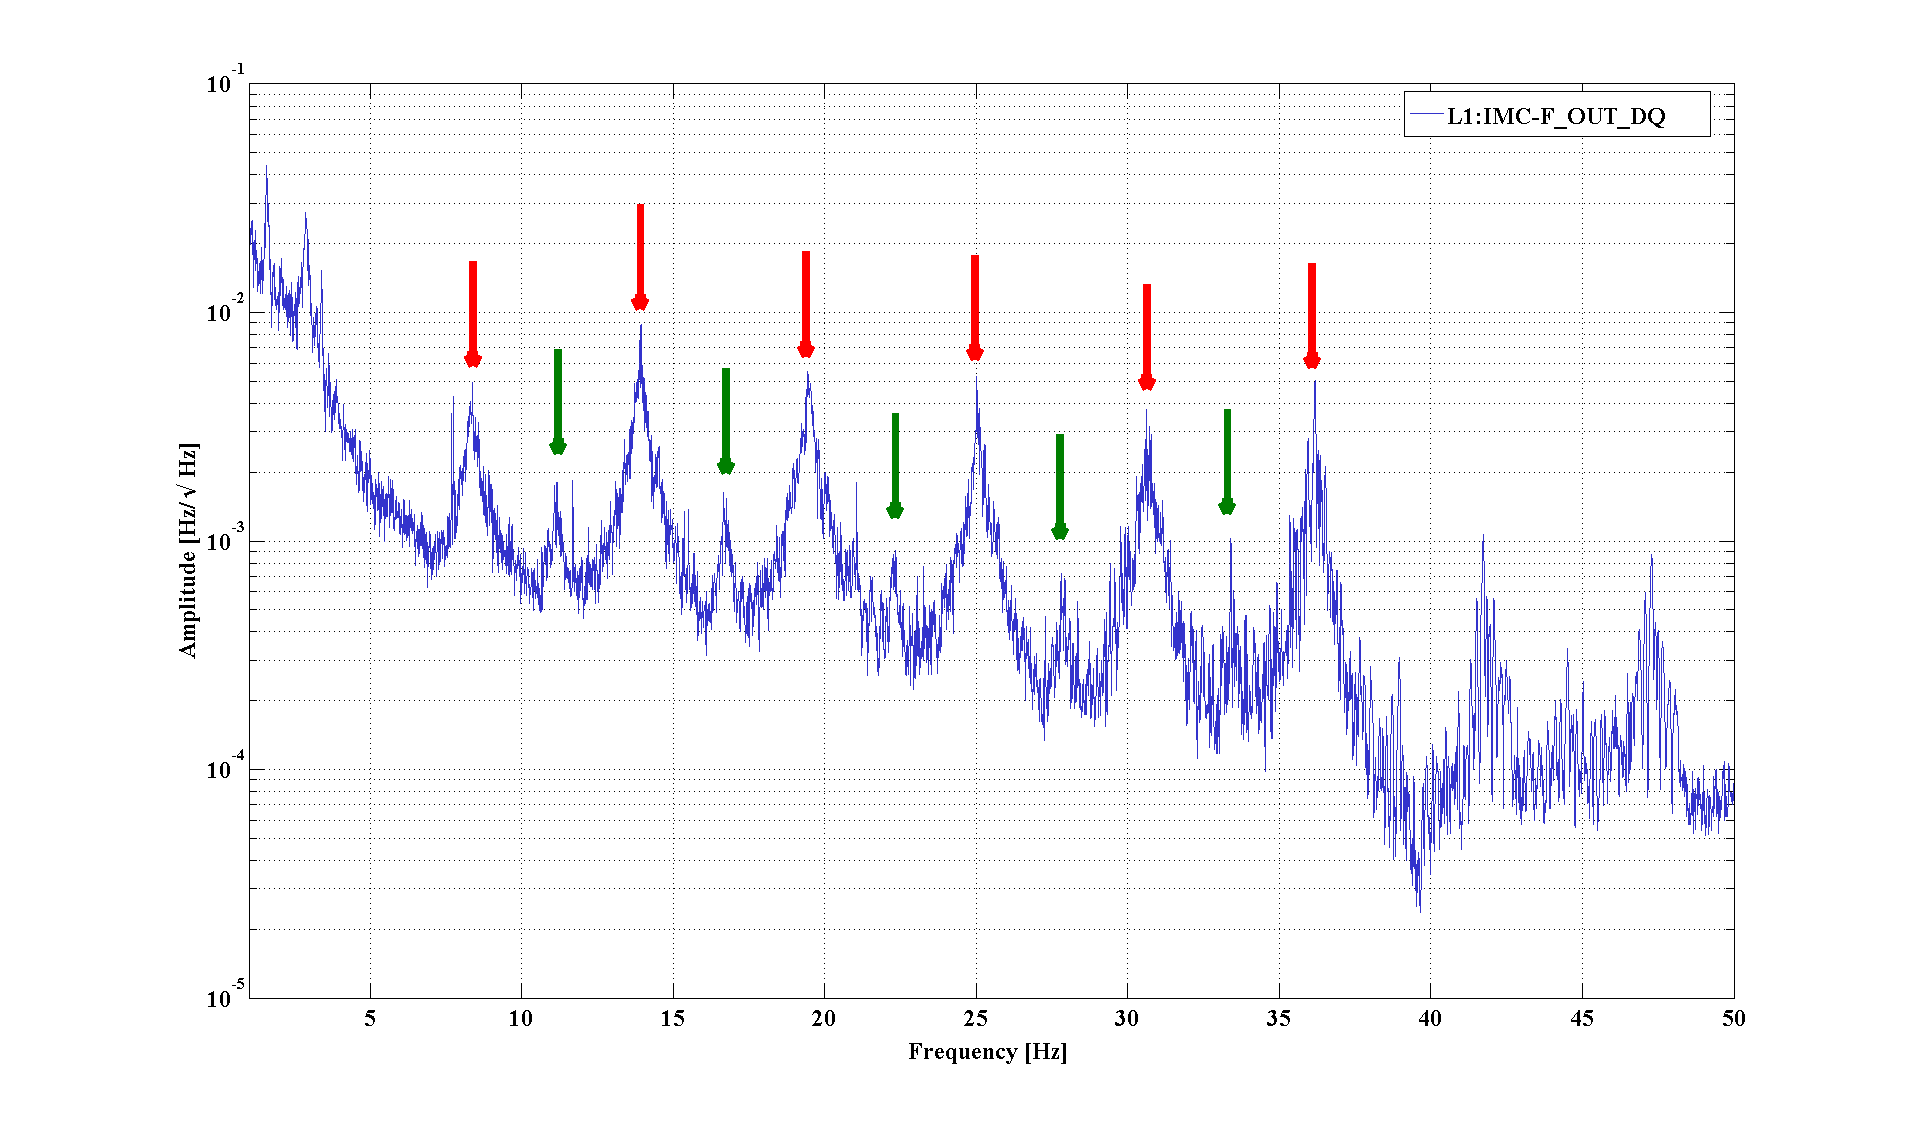
\includegraphics[height=0.6\textwidth]{figures/IMCUpconversion/upconversion_comb.png}
\caption[Spectral comb in IMC control signal]{Spectral comb with a fundamental frequncy of 2.78 Hz in the IMC control signal. Red arrows indicate odd harmonics, green arrows indicate even harmonics. }
\end{figure}

While we have demonstrated that this mechanism is consistent with IMC upconversion noise, 
it has not yet been fully proven. We are currently looking for a better way to look at 
the IMC error point, which is generated using an analog servo board, during times of 
excess seismic motion instead of the control signal. 
We think the source of the excitation may be a vertical resonance of the triple 
pendulum suspension that houses the IMC optics being rung up by the excess motion.

\section{Conclusions}

We found that injecting sinusoidal cavity motion into our input mode cleaner PDH model 
generates an error signal with non-linear spectral artifacts, specifically harmonics 
of the injection frequency, if the cavity motion exceeds the linear PDH range. 
For cavity motion that is symmetric about the locking point of the error signal, 
we find that the error signal contains only odd harmonics. For asymmetric cavity 
motion we find both even and odd harmonics, where the odd harmonics are typically higher 
in amplitude. In such a case, the amplitude of the even harmonics increases as the 
offset from the nominal locking point increases, that is, as the cavity motion is 
more asymmetric.

